% requer: longtable, booktabs, array, graphicx
\subsection{Contextos e o que cada um possui}
O sistema divide-se em cinco contextos delimitados. Cada um tem a sua parte da linguagem ubíqua: o mesmo termo pode querer dizer coisas diferentes consoante o contexto, e é por isso que os contextos estão separados.

\begin{longtable}{@{}p{2.4cm}p{2.9cm}p{3.5cm}p{4.6cm}p{1.9cm}@{}}
\caption{Contextos delimitados do Roamly.}\label{tab:contextos}\\
\toprule \textbf{Contexto} & \textbf{Responsabilidade} & \textbf{Possui} & \textbf{Regras que garante} & \textbf{Histórias} \\ \midrule \endfirsthead
\toprule \textbf{Contexto} & \textbf{Responsabilidade} & \textbf{Possui} & \textbf{Regras que garante} & \textbf{Histórias} \\ \midrule \endhead
\textbf{Planeamento da viagem} & Monta a proposta de viagem e diz quanto custa por pessoa. & Viagem (raiz do agregado), Ideia, Orçamento, Proposta, Opção (voo, alojamento, atividade), Preço e Total por pessoa. & O total por pessoa soma só as opções não cortadas e inclui o transporte até ao aeroporto; os extras que o site esconde aparecem \guillemotleft{}por confirmar\guillemotright{}, nunca são omitidos; o Roamly avisa quando o total passa o limite por pessoa. & US-01, 02, 04, 05, 06, 07, 09, 10, 11, 12, 14, 26, 28, 29 \\ \midrule
\textbf{Vigilância de preços} & Volta a ler continuamente as ligações guardadas e avisa quando o preço sobe. & Oferta vigiada, Leitura de preço e Alerta de preço. & Um alerta mostra só de quanto o preço subiu, sem mensagens de urgência; se a oferta deixa de ser legível, avisa que o preço pode estar desatualizado; o Roamly não congela preços nem reserva. & US-08 (e a leitura automática das US-04 e US-05) \\ \midrule
\textbf{Decisão do grupo} & Recolhe o que cada pessoa pensa e regista o que o grupo combinou. & Grupo, Membro, Coordenador (o(a) organizador(a) das histórias), Opinião, Disponibilidade e Decisão (com prazo). & Um grupo tem exatamente um coordenador; o coordenador vê em que itens há divergência e quem ainda não respondeu; a decisão fica registada mesmo que faltem respostas, e todos os membros a veem. & US-15, 16, 17, 18, 31 \\ \midrule
\textbf{Acerto de pagamentos} & Calcula quanto cada pessoa deve e acompanha quem já pagou. & Acerto (raiz do agregado), Parte da despesa, Pagamento e Lembrete de pagamento. & Só o coordenador marca um pagamento como feito; se alguém sai do grupo, as partes dos restantes são recalculadas; o Roamly regista pagamentos mas não os processa. & US-20, 21, 22 \\ \midrule
\textbf{Balcão da agência {[A]}} & Dá ao agente de viagens um espaço de trabalho por cliente (só na versão para agências). & Quadro do cliente (raiz do agregado), Pedido do cliente, Lembrete no quadro, Fornecedor e Revisão da proposta. & O cliente não vê a proposta antes de o agente a assinar; um pedido com dados em falta é assinalado antes de se montar a proposta; um fornecedor sem preço aparece \guillemotleft{}sem preço\guillemotright{}, nunca como 0 \texteuro{}. & US-03, 13, 19, 23, 24, 25, 27, 30 \\ \bottomrule
\end{longtable}

\subsection{Termos que mudam de significado}
\begin{longtable}{@{}p{3cm}p{3.6cm}p{8.7cm}@{}}
\caption{Termos cujo significado muda entre contextos.}\label{tab:termos}\\
\toprule \textbf{Termo} & \textbf{Contexto} & \textbf{Significado} \\ \midrule \endfirsthead
\toprule \textbf{Termo} & \textbf{Contexto} & \textbf{Significado} \\ \midrule \endhead
\textbf{Proposta} & Planeamento da viagem & O que se monta: um conjunto de opções com preços e total por pessoa, partilhado numa só ligação e sempre atualizado. \\
 & Decisão do grupo & O que o grupo avalia: é só referida por identificador; sobre ela os membros dão opinião e disponibilidade e dela sai a decisão. \\
 & Acerto de pagamentos & Não existe como proposta: só as opções acordadas interessam, e transformam-se em partes da despesa. \\
 & Balcão da agência & Um documento no modelo da agência, com logótipo, que o cliente só vê depois de o agente o assinar. \\
\midrule
\textbf{Membro} & Decisão do grupo & Pessoa do grupo que dá opinião e indica datas; o coordenador é o membro com o papel de planear. \\
 & Acerto de pagamentos & Devedor de uma parte da despesa; não pode marcar pagamentos. \\
 & Vigilância de preços & Destinatário dos alertas de preço. \\
 & Balcão da agência & Não existe: quem recebe a proposta é o cliente, que não faz parte de nenhum grupo. \\
\midrule
\textbf{Opção} & Planeamento da viagem & Item com preço e estado: candidata, cortada (riscada mas visível) ou acordada. \\
 & Vigilância de preços & Uma oferta vigiada: uma ligação guardada com as leituras de preço feitas. \\
 & Decisão do grupo & Aquilo sobre que se opina (IdDaOpção); o que a opção é não interessa. \\
 & Acerto de pagamentos & Uma opção acordada é um custo a dividir pelo grupo. \\
\midrule
\textbf{Preço} & Planeamento da viagem & Preço final: base mais extras (ex.: bagagem de porão), por pessoa. \\
 & Vigilância de preços & Uma leitura num dado momento; só importa a diferença para a anterior. \\
 & Acerto de pagamentos & O montante devido por cada membro (ex.: 98 \texteuro{}). \\
\midrule
\textbf{Total por pessoa / Parte da despesa} & Planeamento da viagem & Total por pessoa: estimativa que muda sempre que um item muda e se compara com o limite. \\
 & Acerto de pagamentos & Parte da despesa: valor fixado depois de as opções serem acordadas, com o total que o coordenador tem de adiantar. \\
\midrule
\textbf{Reservar} & Decisão do grupo e Acerto & O Roamly não reserva: \guillemotleft{}reservar\guillemotright{} é o coordenador sair do Roamly e reservar no site do fornecedor. \\
\bottomrule
\end{longtable}

\subsection{Mapa de contextos}
\begin{figure}[htbp]
\centering
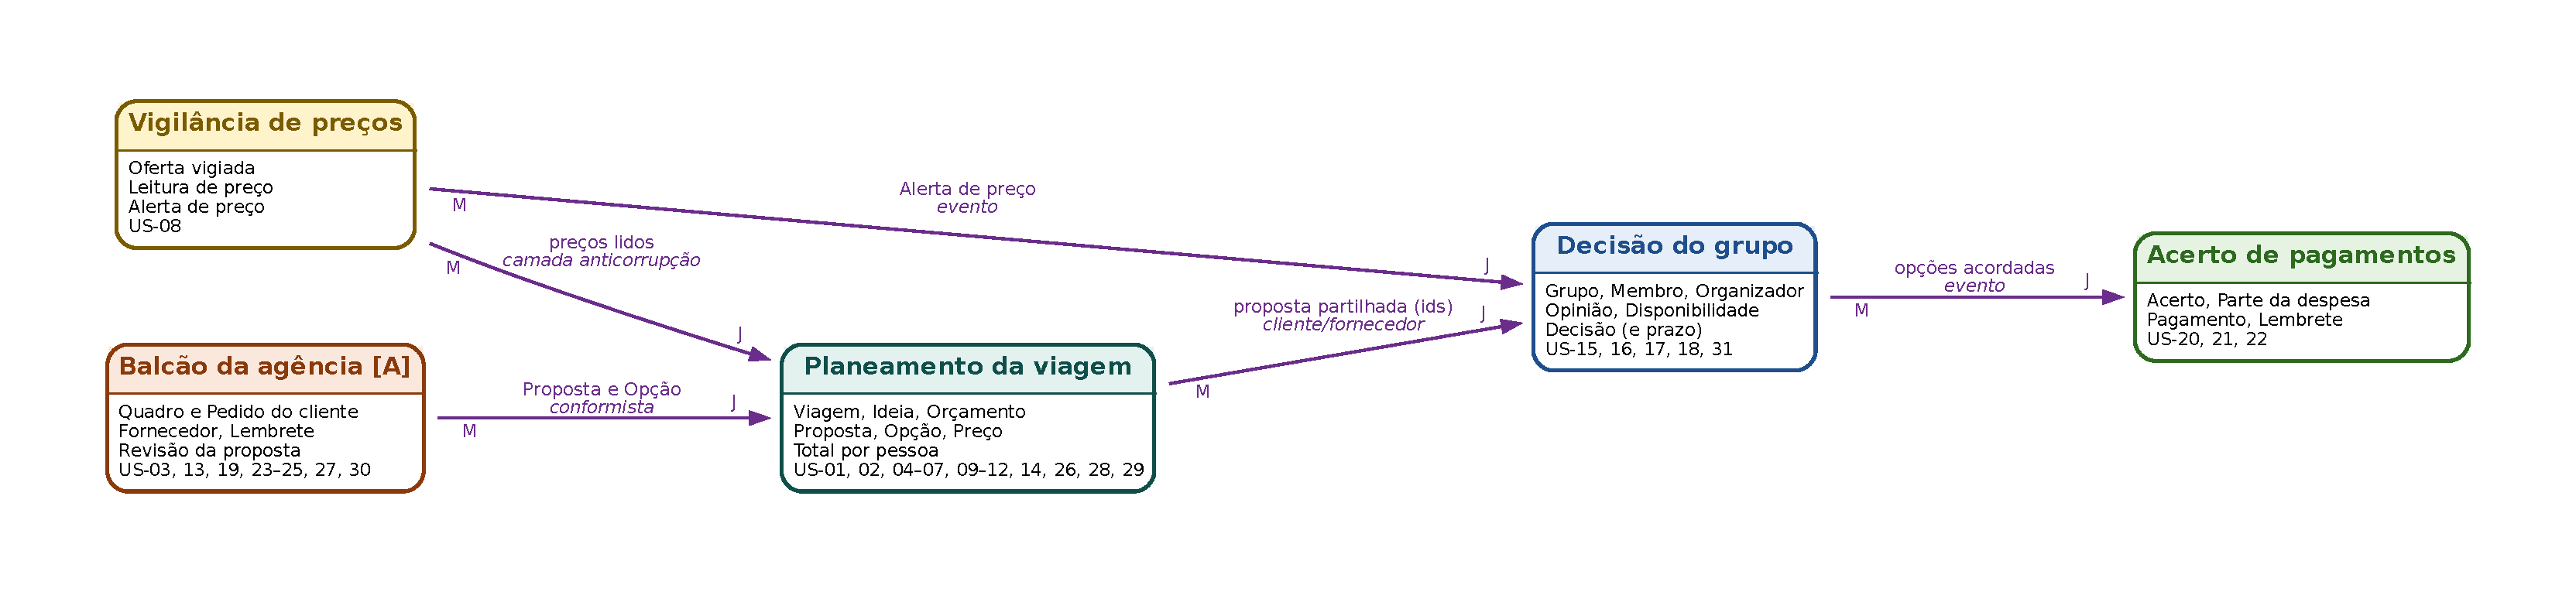
\includegraphics[width=\linewidth]{mapa_de_contextos.pdf}
\caption{Mapa de contextos. M = a montante (fornece), J = a jusante (consome).}
\label{fig:mapa-contextos}
\end{figure}

\begin{longtable}{@{}p{2.3cm}p{2.3cm}p{2.5cm}p{6.1cm}p{1.9cm}@{}}
\caption{Relações entre contextos.}\label{tab:relacoes}\\
\toprule \textbf{A montante} & \textbf{A jusante} & \textbf{Relação} & \textbf{O que passa} & \textbf{Histórias} \\ \midrule \endfirsthead
\toprule \textbf{A montante} & \textbf{A jusante} & \textbf{Relação} & \textbf{O que passa} & \textbf{Histórias} \\ \midrule \endhead
Vigilância de preços & Planeamento da viagem & Camada anticorrupção (no Planeamento) & Os preços lidos nos sites passam a ser o Preço de uma Opção; se a página não for legível, o coordenador preenche à mão. & US-04, 05, 08 \\
Planeamento da viagem & Decisão do grupo & Cliente/Fornecedor & A proposta partilhada; a Decisão do grupo só guarda IdDaProposta e IdDaOpção e vê sempre a versão atualizada. & US-14, 15, 16 \\
Vigilância de preços & Decisão do grupo & Evento publicado & O Alerta de preço chega a todos os membros do grupo, haja ou não prazo. & US-08 \\
Decisão do grupo & Acerto de pagamentos & Evento publicado & As opções acordadas dão origem às partes da despesa. & US-18, 20 \\
Balcão da agência & Planeamento da viagem & Conformista & A agência usa Proposta e Opção tal como o Planeamento as define e acrescenta revisão, assinatura e fornecedores; o preço das ofertas guardadas chega-lhe por aqui. & US-13, 23, 30 \\
Todos & Todos & Núcleo partilhado (pequeno) & Dinheiro e identificadores (IdDoGrupo, IdDoMembro, IdDaProposta, IdDaOpção). & — \\
\bottomrule
\end{longtable}
